\documentclass{article}
\usepackage{caption}
\usepackage{subcaption}
\usepackage{tikz}
\usetikzlibrary{knots,calc}
\begin{document}
\begin{figure}
  \begin{subfigure}[b]{0.45\textwidth}
    \centering
    \resizebox{\linewidth}{!}{
      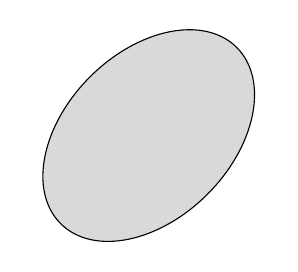
\begin{tikzpicture}
    \draw[rotate=-45,fill=gray!30] (0,0) ellipse (30pt and 45pt);
    %\draw (current bounding box.south east) rectangle (current bounding box.north west);
    \end{tikzpicture}    }
    \caption{Convex Set}
    \label{a}
  \end{subfigure}
  \begin{subfigure}[b]{0.45\textwidth}
    \centering
    \resizebox{\linewidth}{!}{
    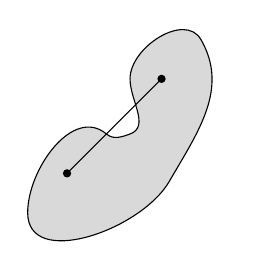
\begin{tikzpicture}
    \useasboundingbox (-1,-1.35) rectangle (1.5,1.35); % values found by trial and error
    \draw[fill=gray!30] (0,0) to [out=140,in=90] (-1,-1)
    to [out=-90,in=240] (0.8,-0.6)
    to [out=60,in=-60] (1.2,1.2)
    to [out=120,in=90] (0.3,0.7)
    to [out=-90,in=20] (0.3,0)
    to [out=200,in=-40] (0,0);
    \draw (-0.5,-0.5) -- (0.7,0.7);
    \fill (-0.5,-0.5) circle[radius=1.5pt];
    \fill (0.7,0.7) circle[radius=1.5pt];
    %\draw (current bounding box.south east) rectangle (current bounding box.north west);
    \end{tikzpicture}
    }
    \caption{Non-convex set}
    \label{b}
  \end{subfigure}
\caption{Examples of convex and non-convex sets.}
\end{figure}
\end{document}